\documentclass[a4]{article}
\usepackage[utf8]{inputenc}
\usepackage{hyperref}
\usepackage{graphicx}
\usepackage{url}
\usepackage{subcaption}
\usepackage{xspace} 
\usepackage{setspace}
\title{Criterion B – Design}
\begin{document}
\doublespacing
%\maketitle
%\newpage
My client (Yerken Shantayev) wants an application with friendly interface and it should be easy to use. He doesn’t want to write all calculations and reports by hand as shown in Figure \ref{fig:old} below.\\

\begin{figure}[h!]
\begin{center}
  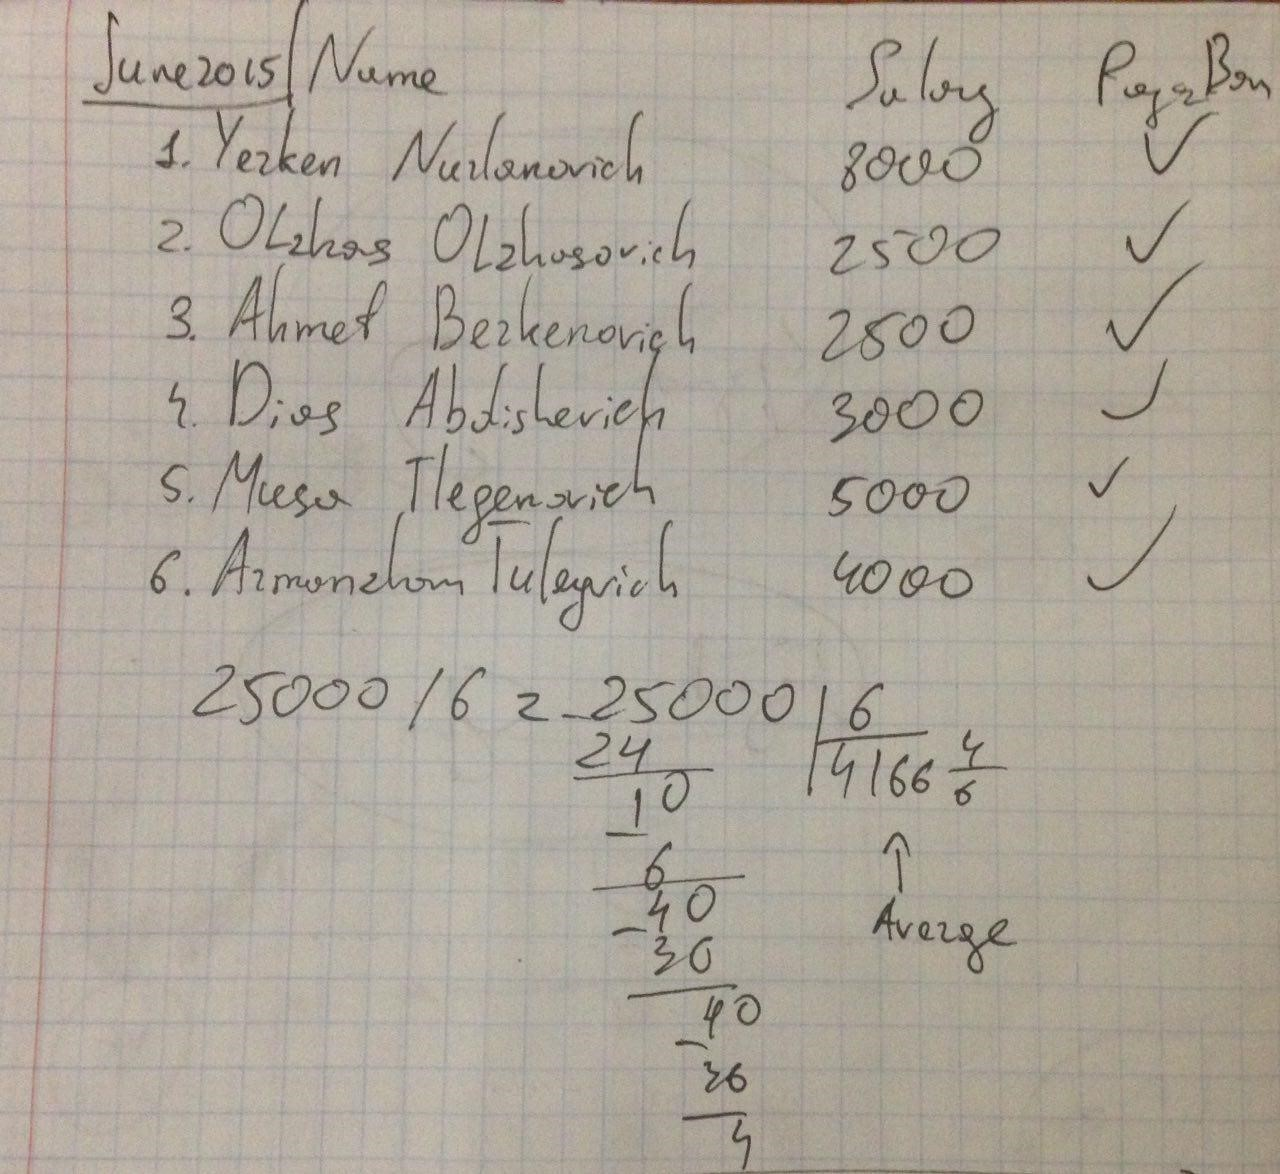
\includegraphics[width=0.75\textwidth]{old.jpg}
  \caption{Method that the client uses to calculate salaries for his employees.}
  \label{fig:old}
\end{center}
\end{figure}

The name of the application- “Salary Calculator”. One of the main requirements of any application is design. It should be simple, easy to navigate and user-friendly. My client – Yerken Shantayev wanted an application, where he would be able to add, edit, and remove records about employees. Manage the salary and premium budget. Save all information into one plain text file for later use.\\
In order to make it easy to use, I have divided the main form into 3 groups. \\
The first one, on the left side, is a list view item list and four main buttons: add, edit, remove or sort the list of employees.\\
The second group is located in the middle of the form. It contains all input text boxes, education checkbox and upload image option. Also, all budget preferences, as overall budget and premium option are located in the bottom of the middle group.\\
The third and final group is located on the right side of the form and the content of this group is connected with the data analysis and data representation. The user will be able to see all the statistics data, the options are average salary, median, standard deviation, IQR, lower and upper quartile. Also, a button to open salary graph or load all the processed data into a plain text file. I discussed the prototype below with my client, he liked it. The sketch of GUI is shown below in Figure \ref{fig:plan}.\\

\begin{figure}[h!]
\begin{center}
  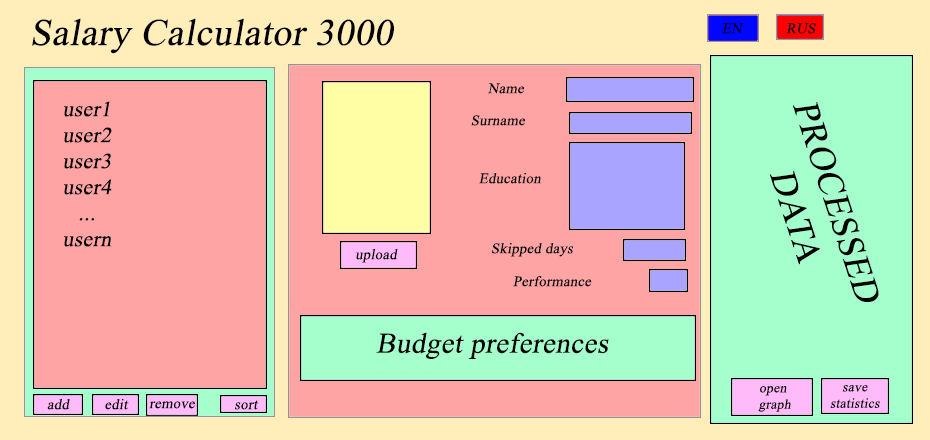
\includegraphics[width=\textwidth]{plan.png}
  \caption{The schematic prototype of the design of the application “Salary Calculator”.}
  \label{fig:plan}
\end{center}
\end{figure}

The diagram in Figure \ref{fig:flow} shows how the data is "flowing" and events are happening during the application execution.\\

The diagram in Figure \ref{fig:modular} shows how the application is divided in terms of forms, pages, options and events.\\

As an OOP approach at the problem, a class “employeeClass” will be created and it will store the characteristics and data about each employee in the database. Therefore, dividing the code into modules and classes will make the application easier to develop and test it.\\
Figure \ref{subf:add} shows an algorithm of adding a new record into the database. This happens, when the user clicks the “Add” button.\\

The Figure \ref{subf:calc} below shows the most important function in the application – salary calculation. When the “Calculate” button is pressed, it goes through validation processes. After that, each employee gets his own salary and premium. The database and statistics section are being updated.

\begin{figure}[ht]
  \centering
  \begin{subfigure}[b]{0.7\linewidth}
    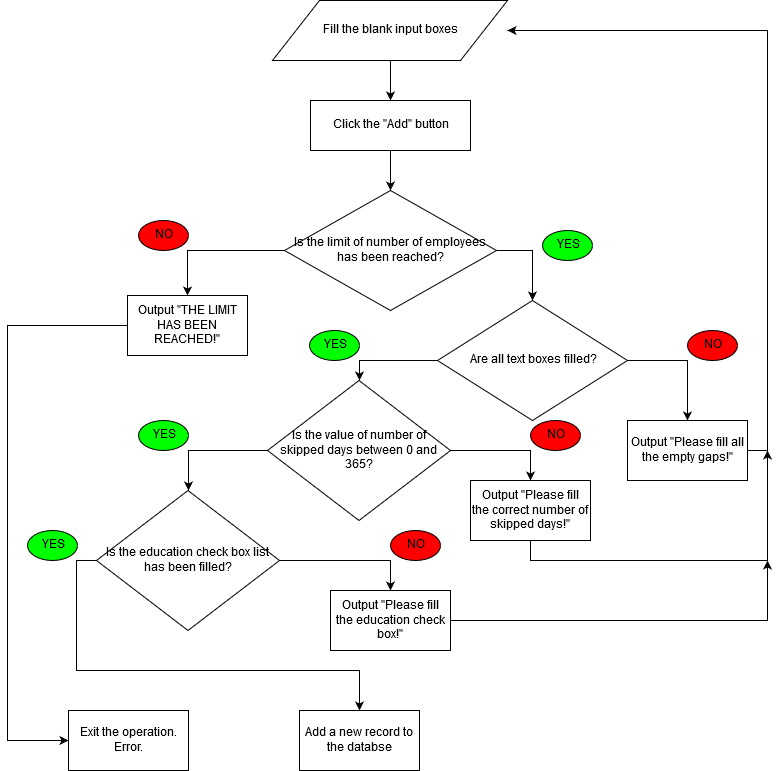
\includegraphics[width=\linewidth]{box.png}
    \caption{System Flowchart, which is showing the algorithm for adding a new record.}
    \label{subf:add}
  \end{subfigure}
  \begin{subfigure}[b]{0.7\linewidth}
    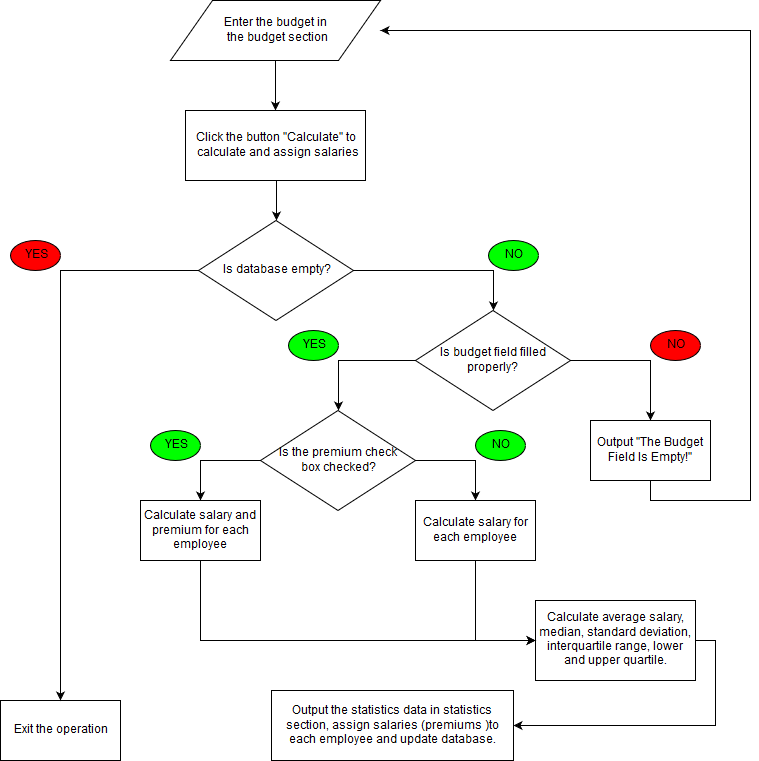
\includegraphics[width=\linewidth]{box2.png}
    \caption{System Flowchart, which is showing the algorithm of salary calculation and assignment.}
    \label{subf:calc}
  \end{subfigure}
  \caption{System Flowcharts of two events.}
  \label{fig:coffee}
\end{figure}


\begin{figure}[ht]
\begin{center}
  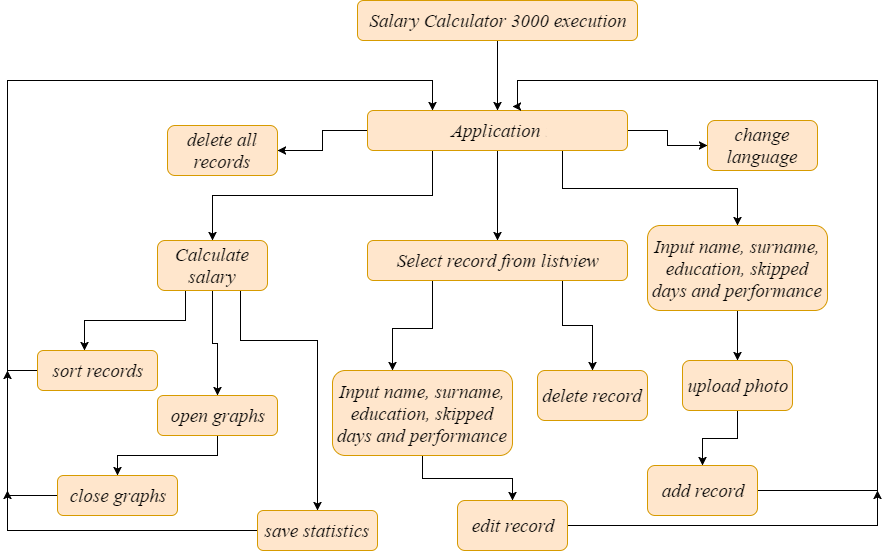
\includegraphics[width=\textwidth]{flow.png}
  \caption{Diagram representing the flow of data and events.}
  \label{fig:flow}
\end{center}
\end{figure}

\begin{figure}[ht]
\begin{center}
  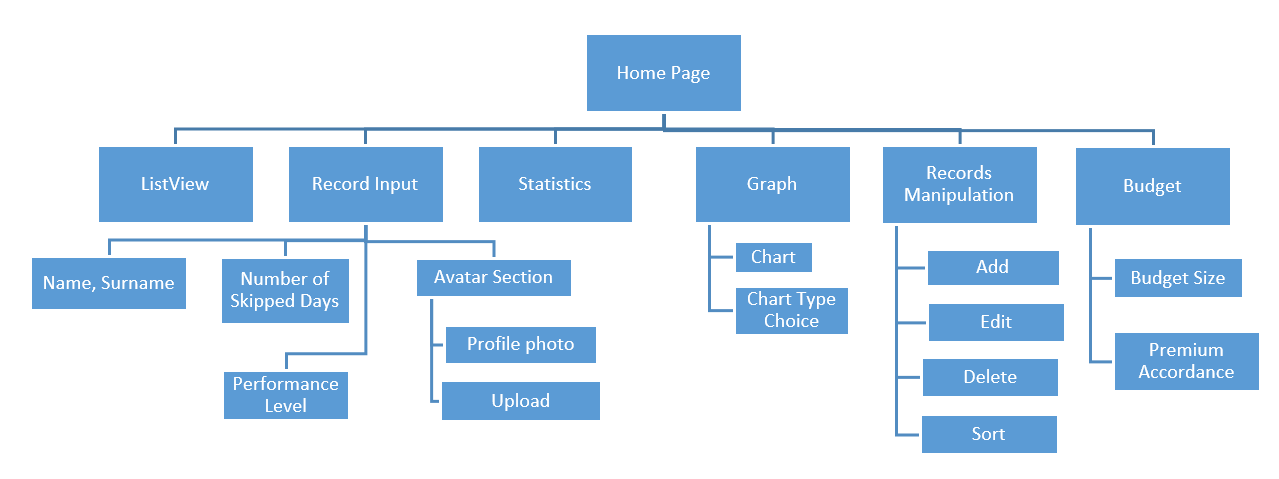
\includegraphics[width=\textwidth]{modular.png}
  \caption{Modular Decomposition of the program.}
  \label{fig:modular}
\end{center}
\end{figure}
\end{document}
